% \renewcommand{\thefigure}{A.\arabic{section}.\arabic{figure}hhh}
\counterwithin{figure}{section}
\setcounter{section}{2} % Assuming section A.3 corresponds to section 3
\setcounter{figure}{0}  % Reset figure counter for this section


\phantomsection
\subsection{Supplementary Plots}


%%%%%%%%%%%%%%%%%%%%
%% SUPPLEMENTARY %%%
%%%%%%%%%%%%%%%%%%%%


\begin{figure}[htbp]
  \centering
  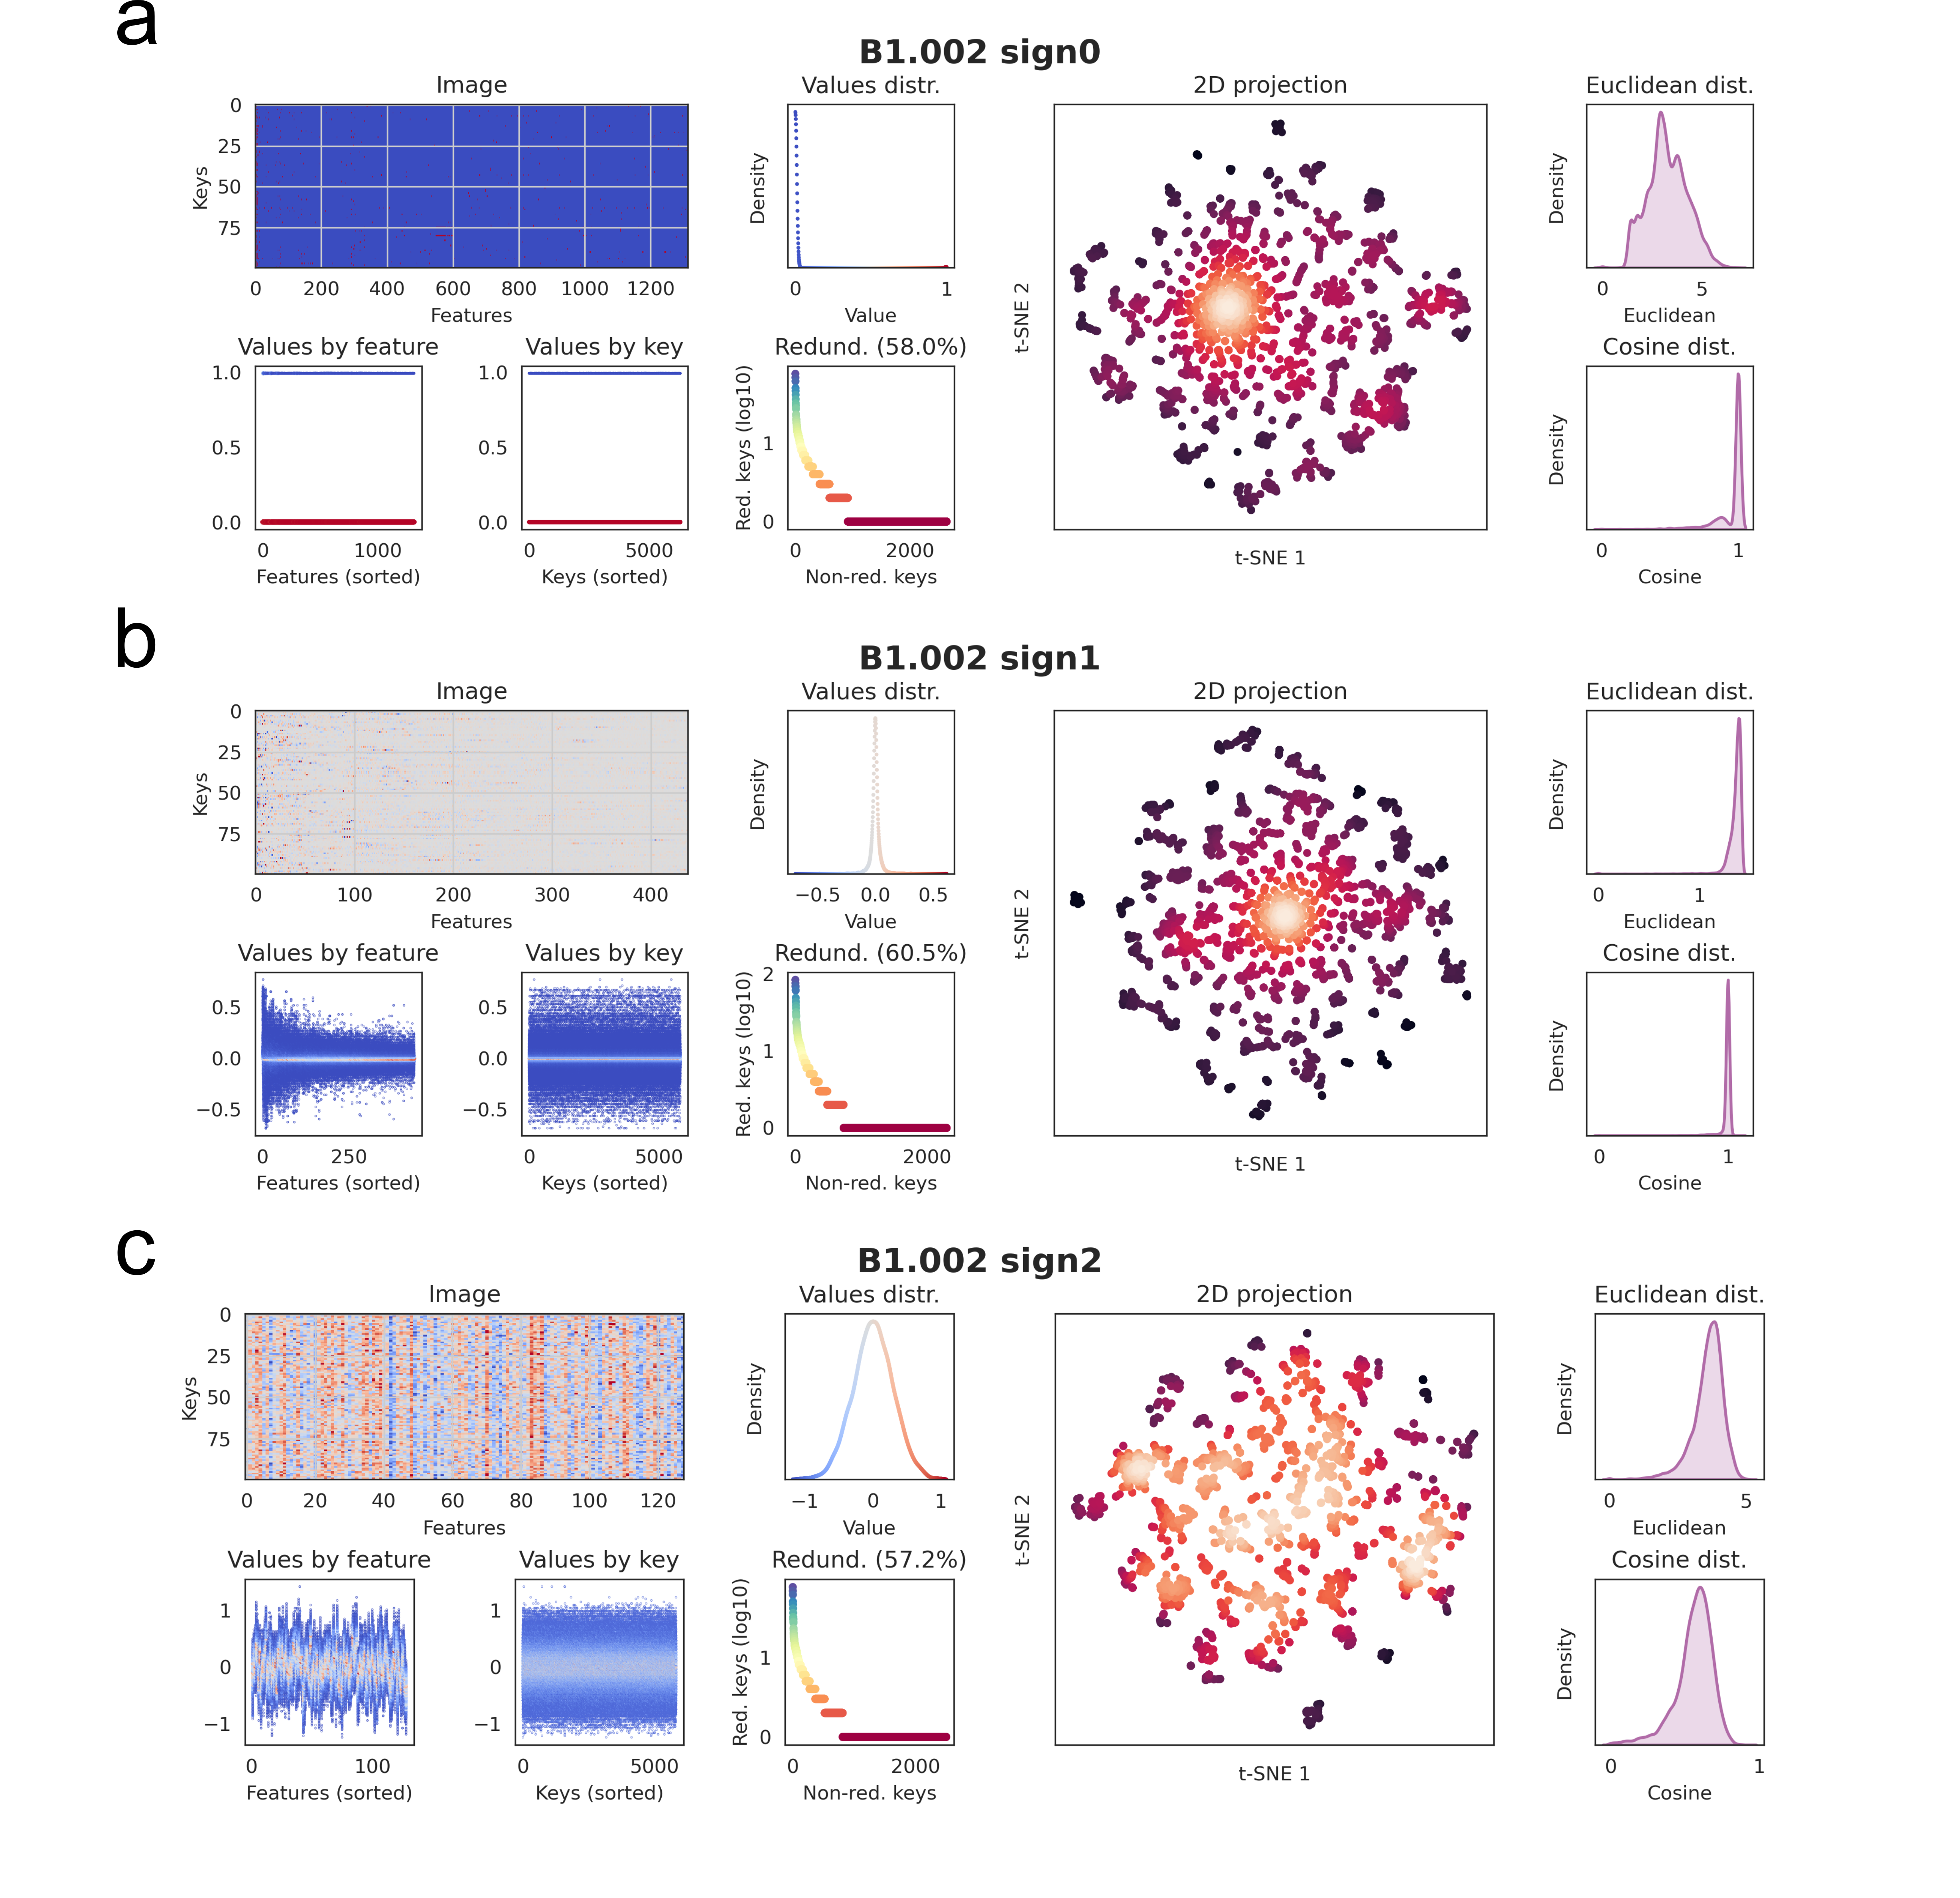
\includegraphics[width=0.9\linewidth]{figures/Protocols/Supplementary/B1.002_v2.png}
  \caption{
    Diagnosis plots for the B1.002 space.
    \textbf{a)} type 0 signatures,
    \textbf{b)} type I signatures,
    \textbf{c)} type II signatures. For further information about diagnosis plots, please see the \hyperref[Supplementary_Protocols_Diagnosis]{Supplementary Information}.
  }
  \label{Protocols_FigS1}
\end{figure}


\begin{figure}[htbp]
  \centering
  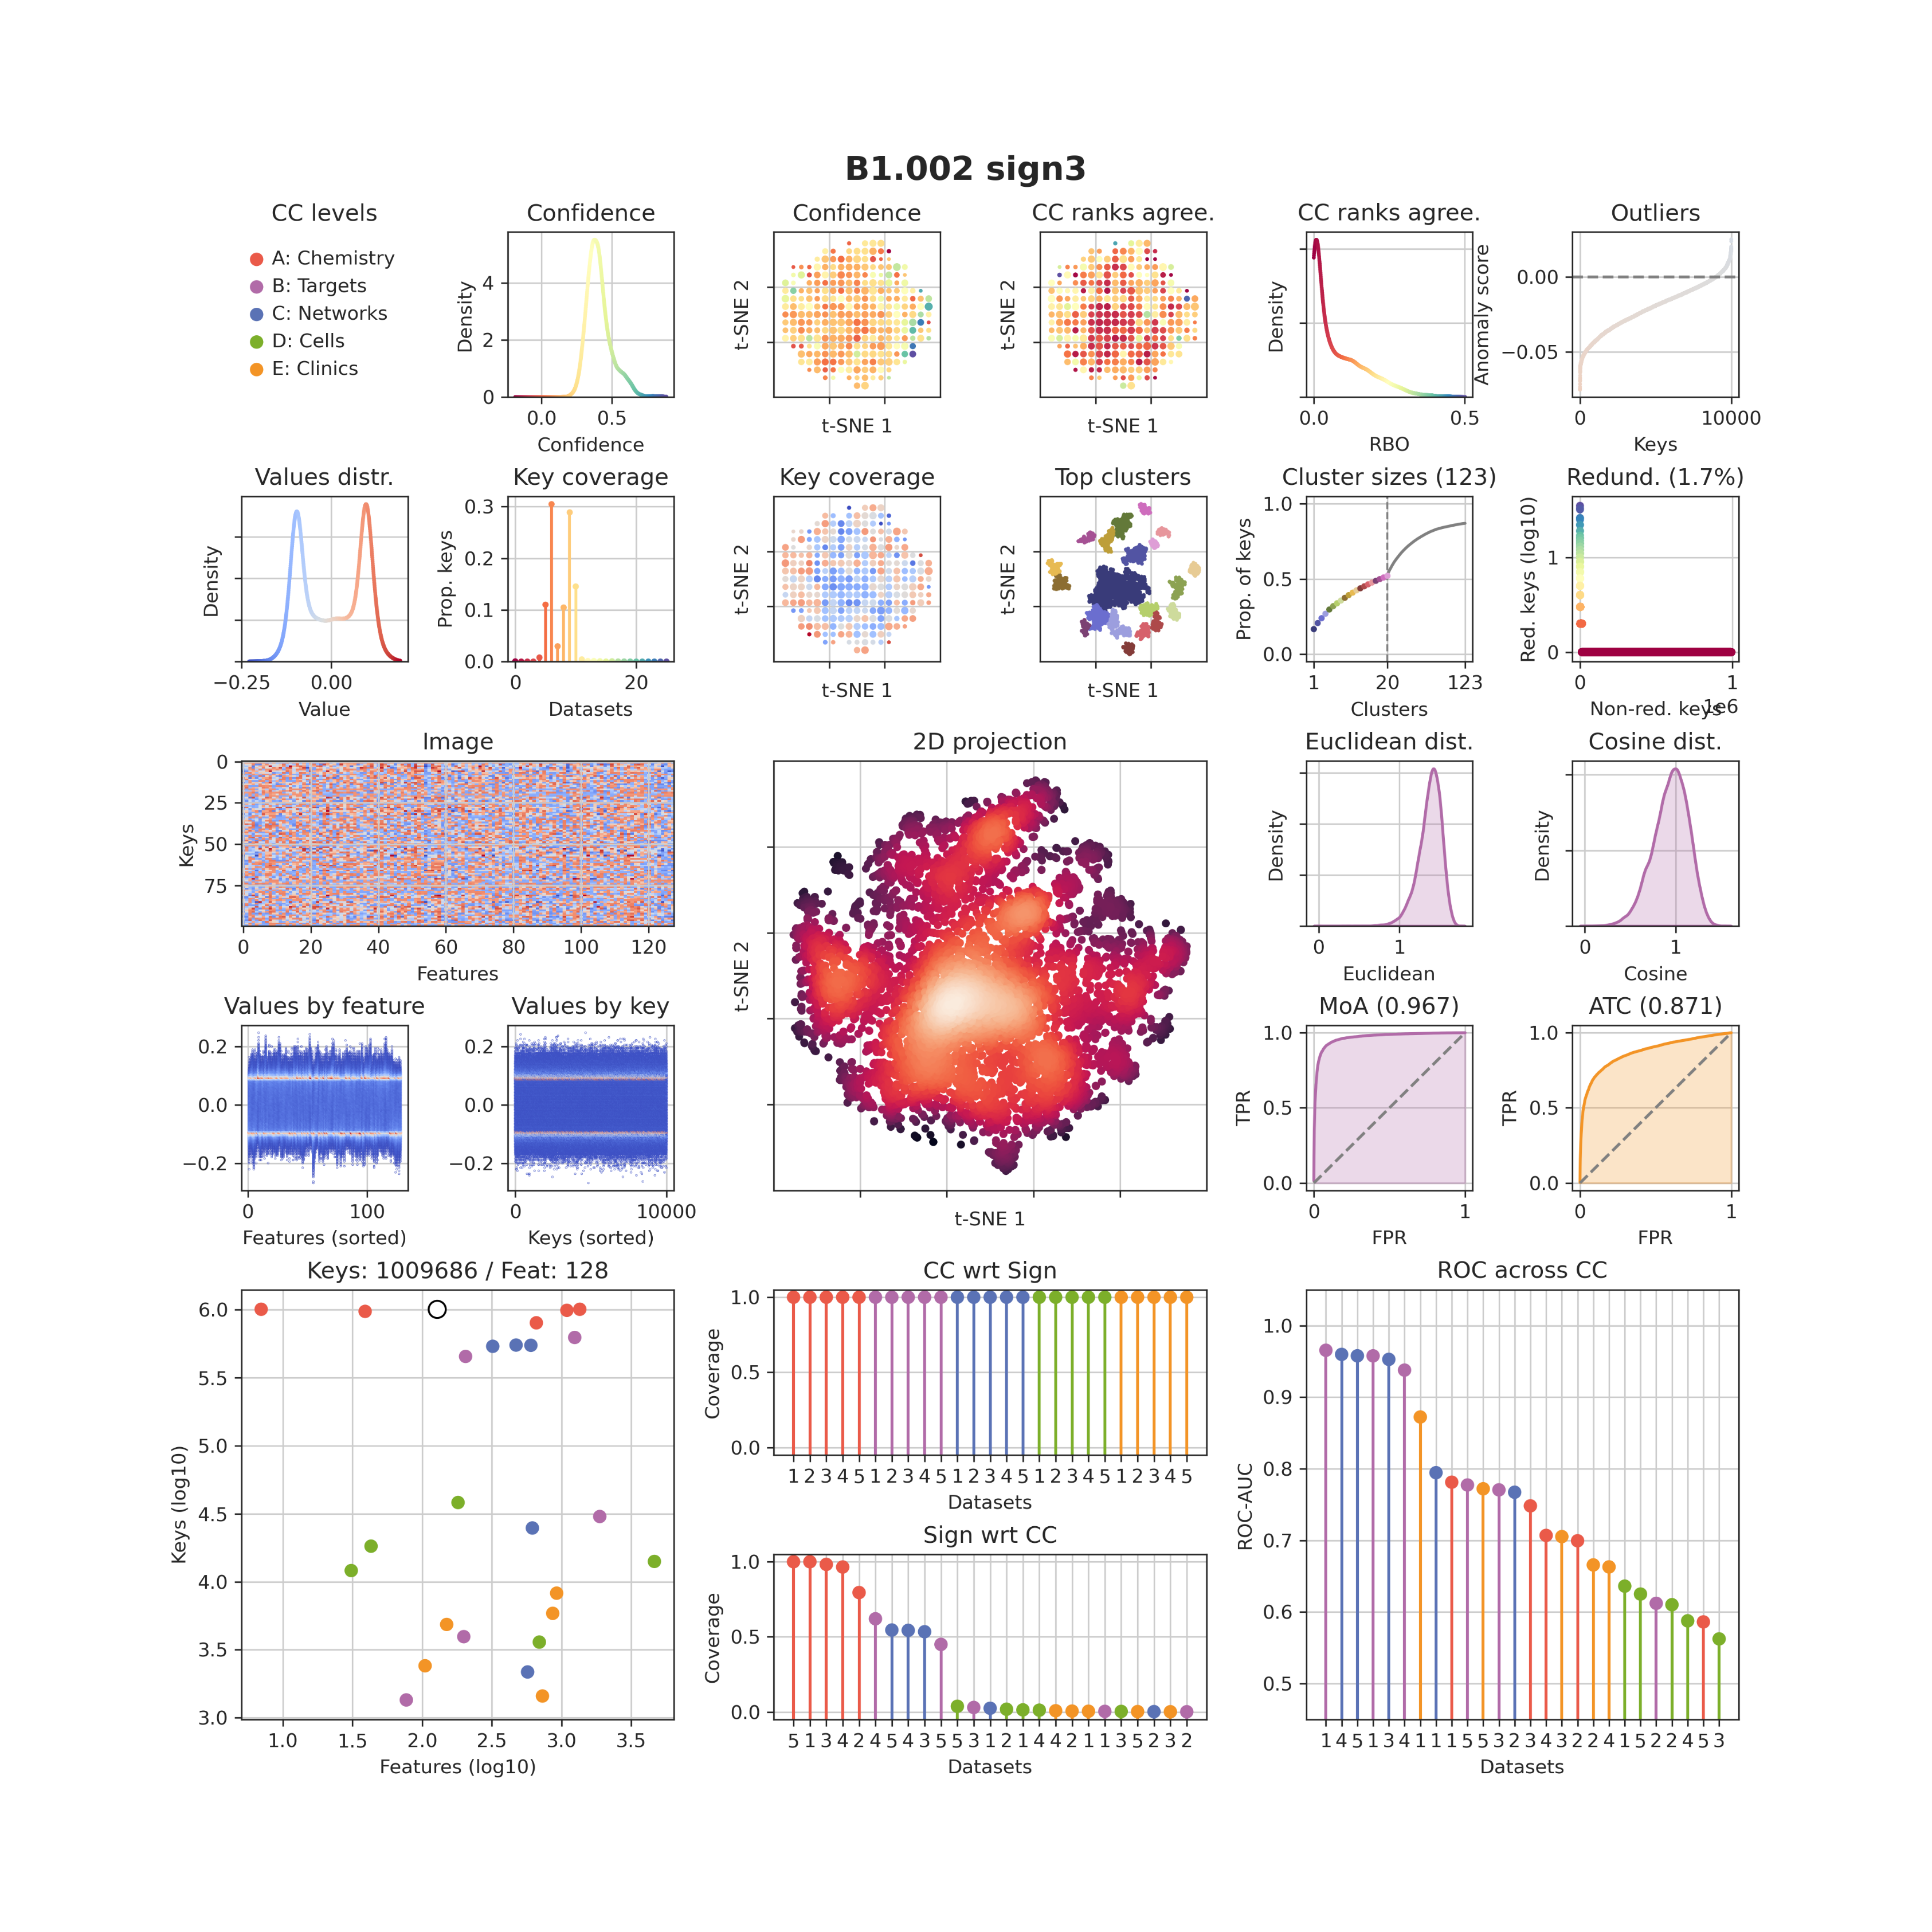
\includegraphics[width=1\linewidth]{figures/Protocols/Supplementary/B1_medium.sign3_v2.png}
  \caption{
    Extended diagnosis plots for B1.002 type III signatures. For further information about diagnosis plots, please see the \hyperref[Supplementary_Protocols_Diagnosis]{Supplementary Information} and check our \href{https://gitlabsbnb.irbbarcelona.org/packages/protocols}{Gitlab repository}.
  }
  \label{Protocols_FigS2}
\end{figure}


\begin{figure}[htbp]
  \centering
  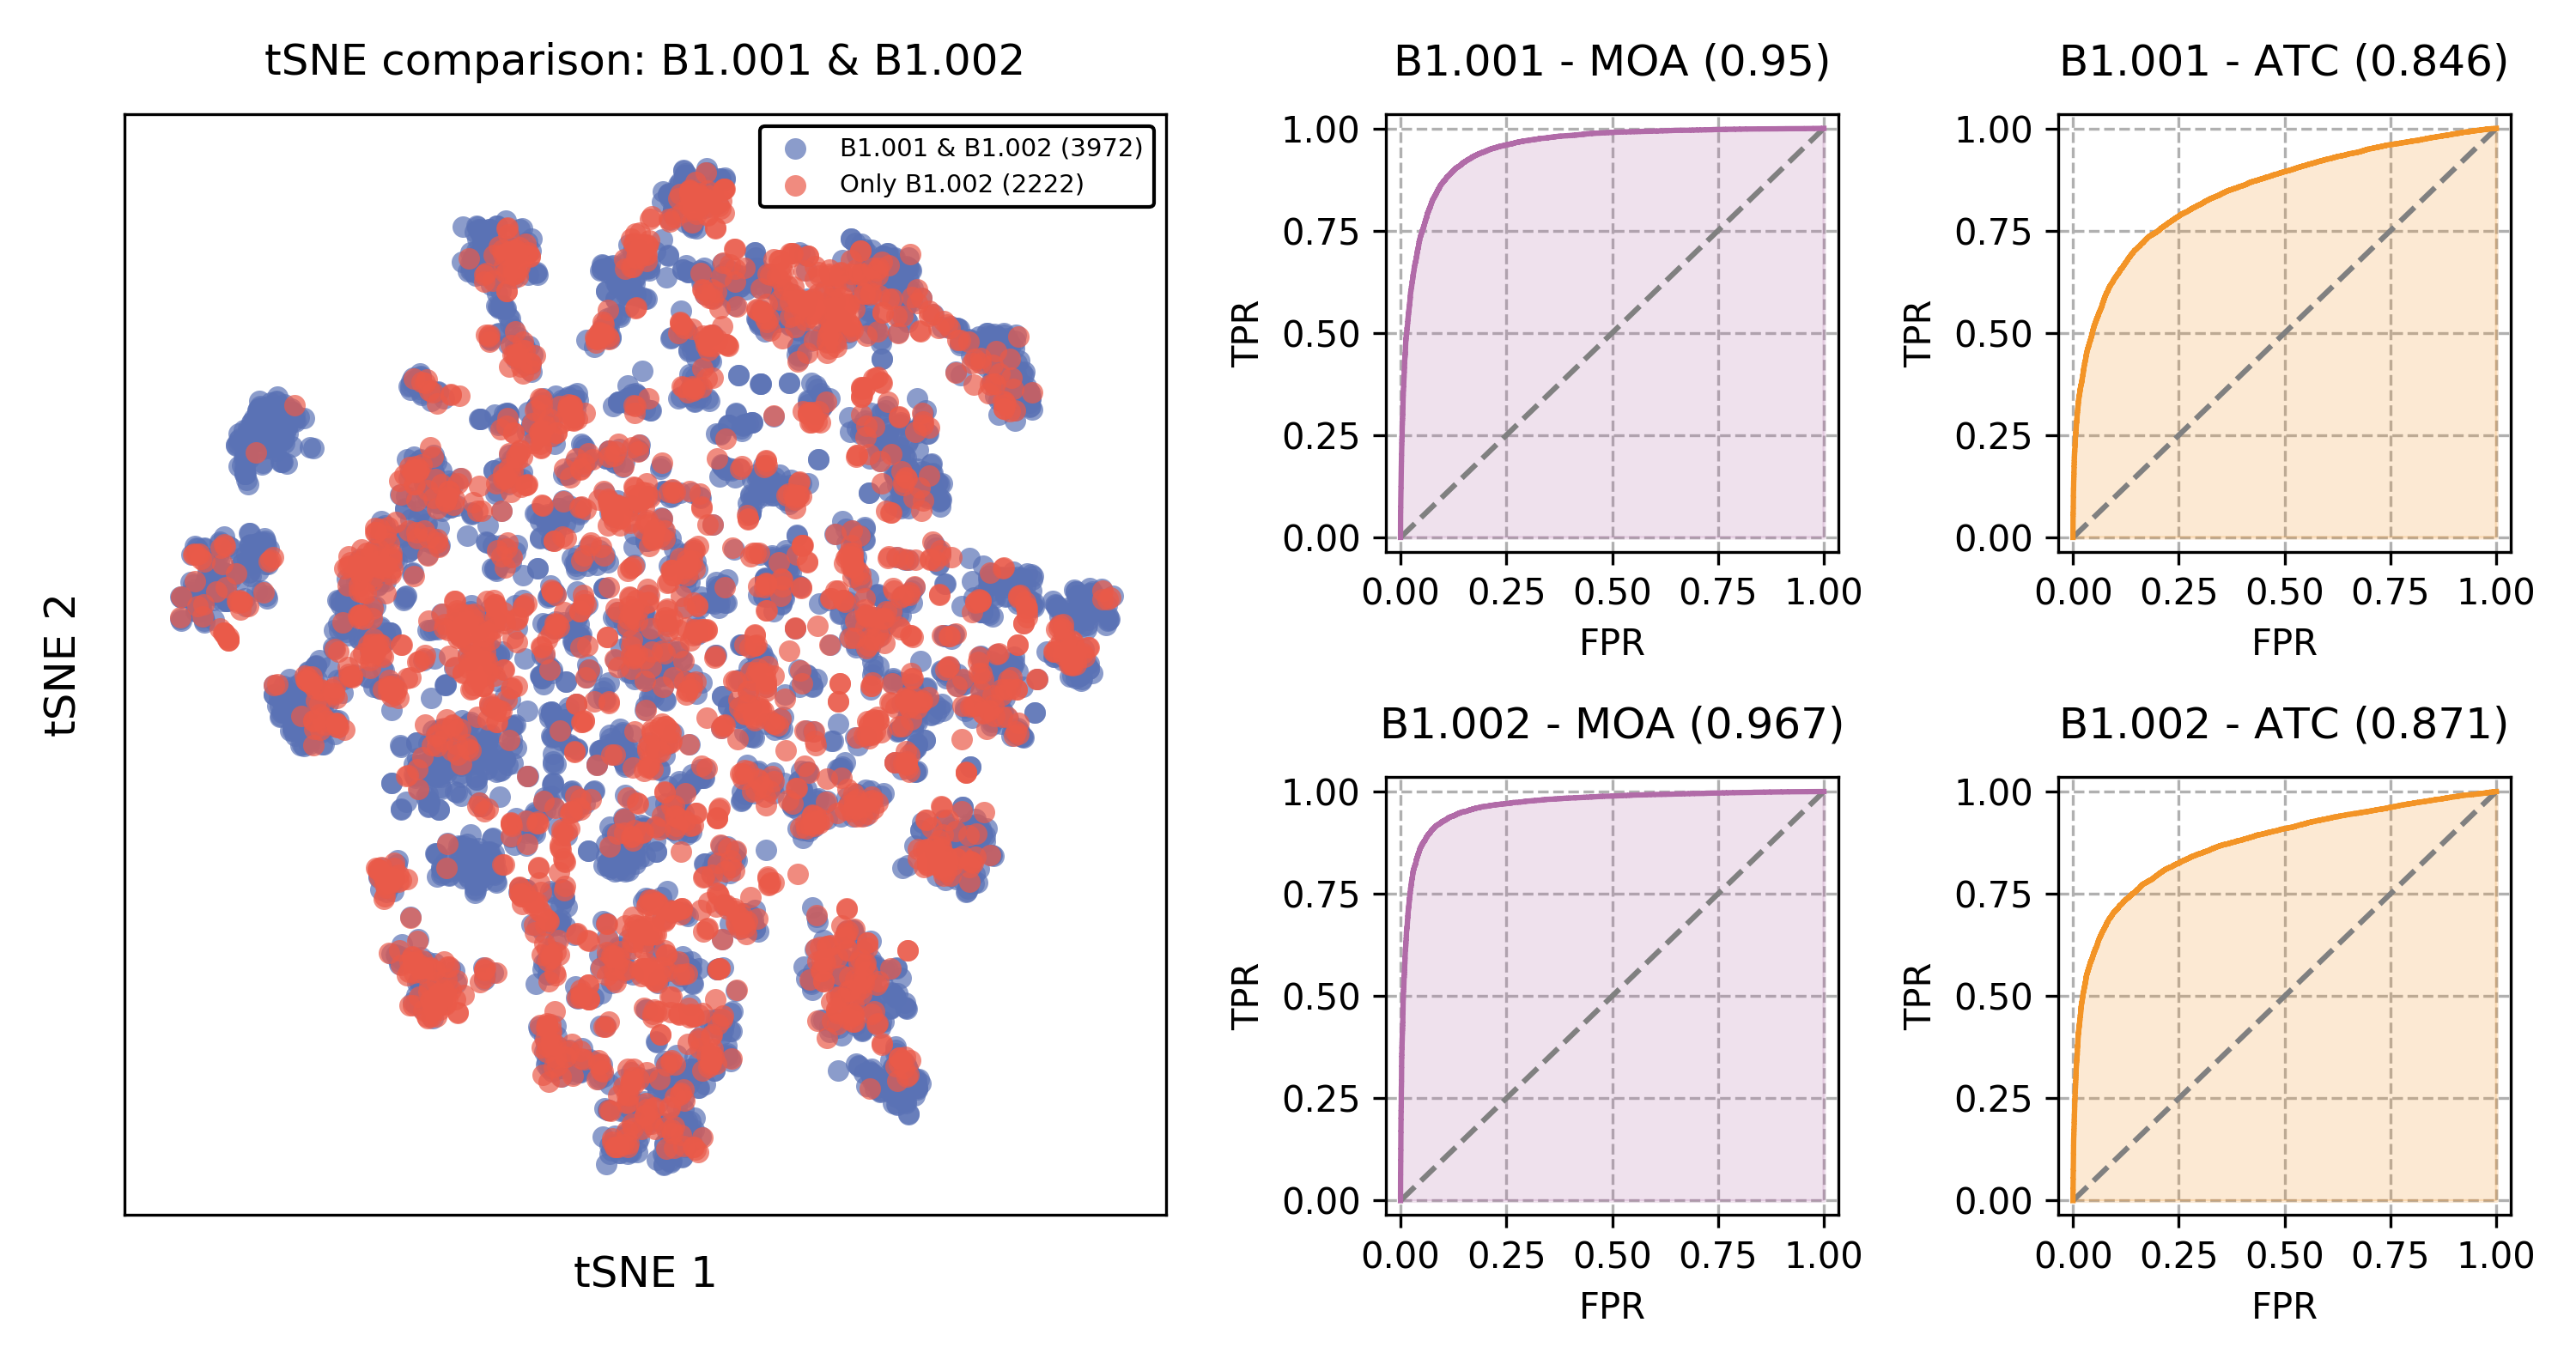
\includegraphics[width=1\linewidth]{figures/Protocols/Supplementary/FigS3.png}
  \caption{
    Comparison between B1.001 and B1.002. Left: 2D tSNE representation of B1.001 and B1.002 type III signatures having a corresponding type 0 signature in B1.001 and B1.002, respectively. Right: recapitulation of MOA (B1.001 type 0 signatures, purple) and ATC (E1.001 type 0 signatures, orange) using B1.001 (top) and B1.002 (bottom) type III signatures. 
  }
  \label{Protocols_FigS3}
\end{figure}


\begin{figure}[htbp]
  \centering
  \includegraphics[width=1\linewidth]{figures/Protocols/Supplementary/D1.002_v2.png}
  \caption{
    Diagnosis plots for the D1.002 space
    \textbf{a)} type 0 signatures,
    \textbf{b)} type I signatures,
    \textbf{c)} type II signatures. For further information about diagnosis plots, please see the \hyperref[Supplementary_Protocols_Diagnosis]{Supplementary Information}.
  }
  \label{Protocols_FigS4}
\end{figure}

\begin{figure}[htbp]
  \centering
  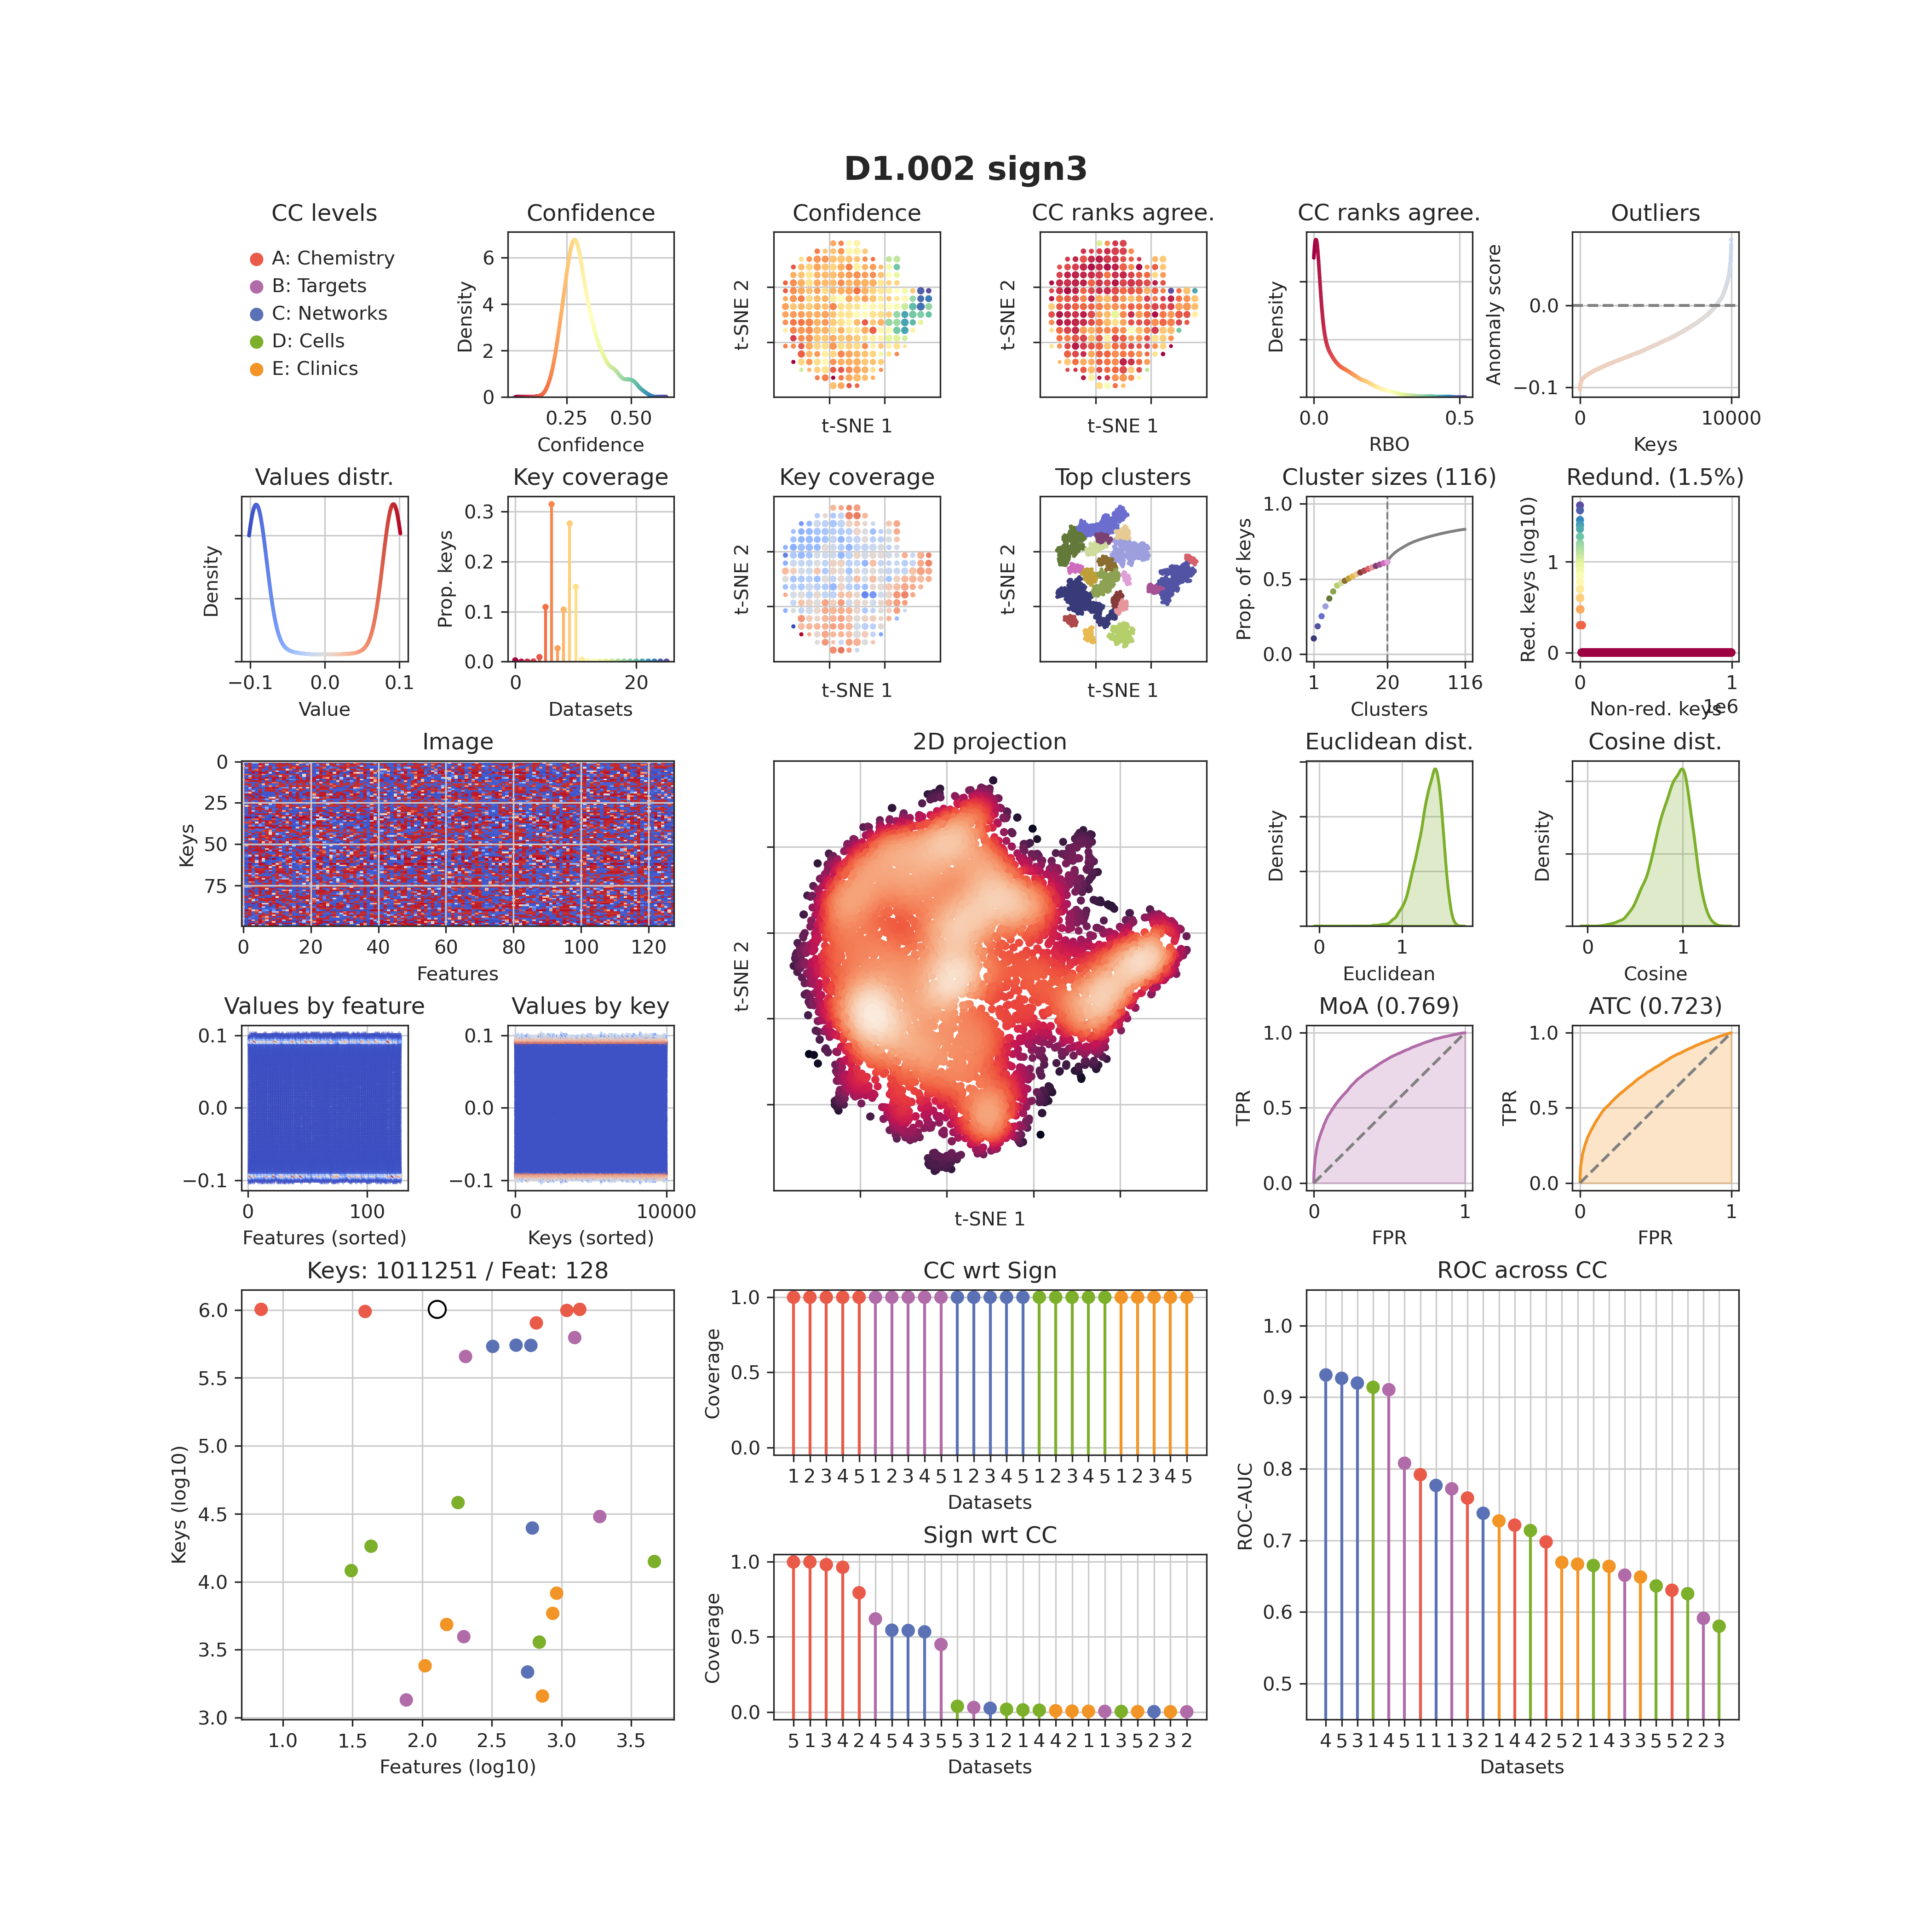
\includegraphics[width=1\linewidth]{figures/Protocols/Supplementary/D1.002_sign3_local_CC_D1_sign0_medium.png}
  \caption{
    Extended diagnosis plots for D1.002 type III signatures. For further information about diagnosis plots, please see the \hyperref[Supplementary_Protocols_Diagnosis]{Supplementary Information} and check our \href{https://gitlabsbnb.irbbarcelona.org/packages/protocols}{Gitlab repository}.
  }
  \label{Protocols_FigS5}
\end{figure}

\begin{figure}[htbp]
  \centering
  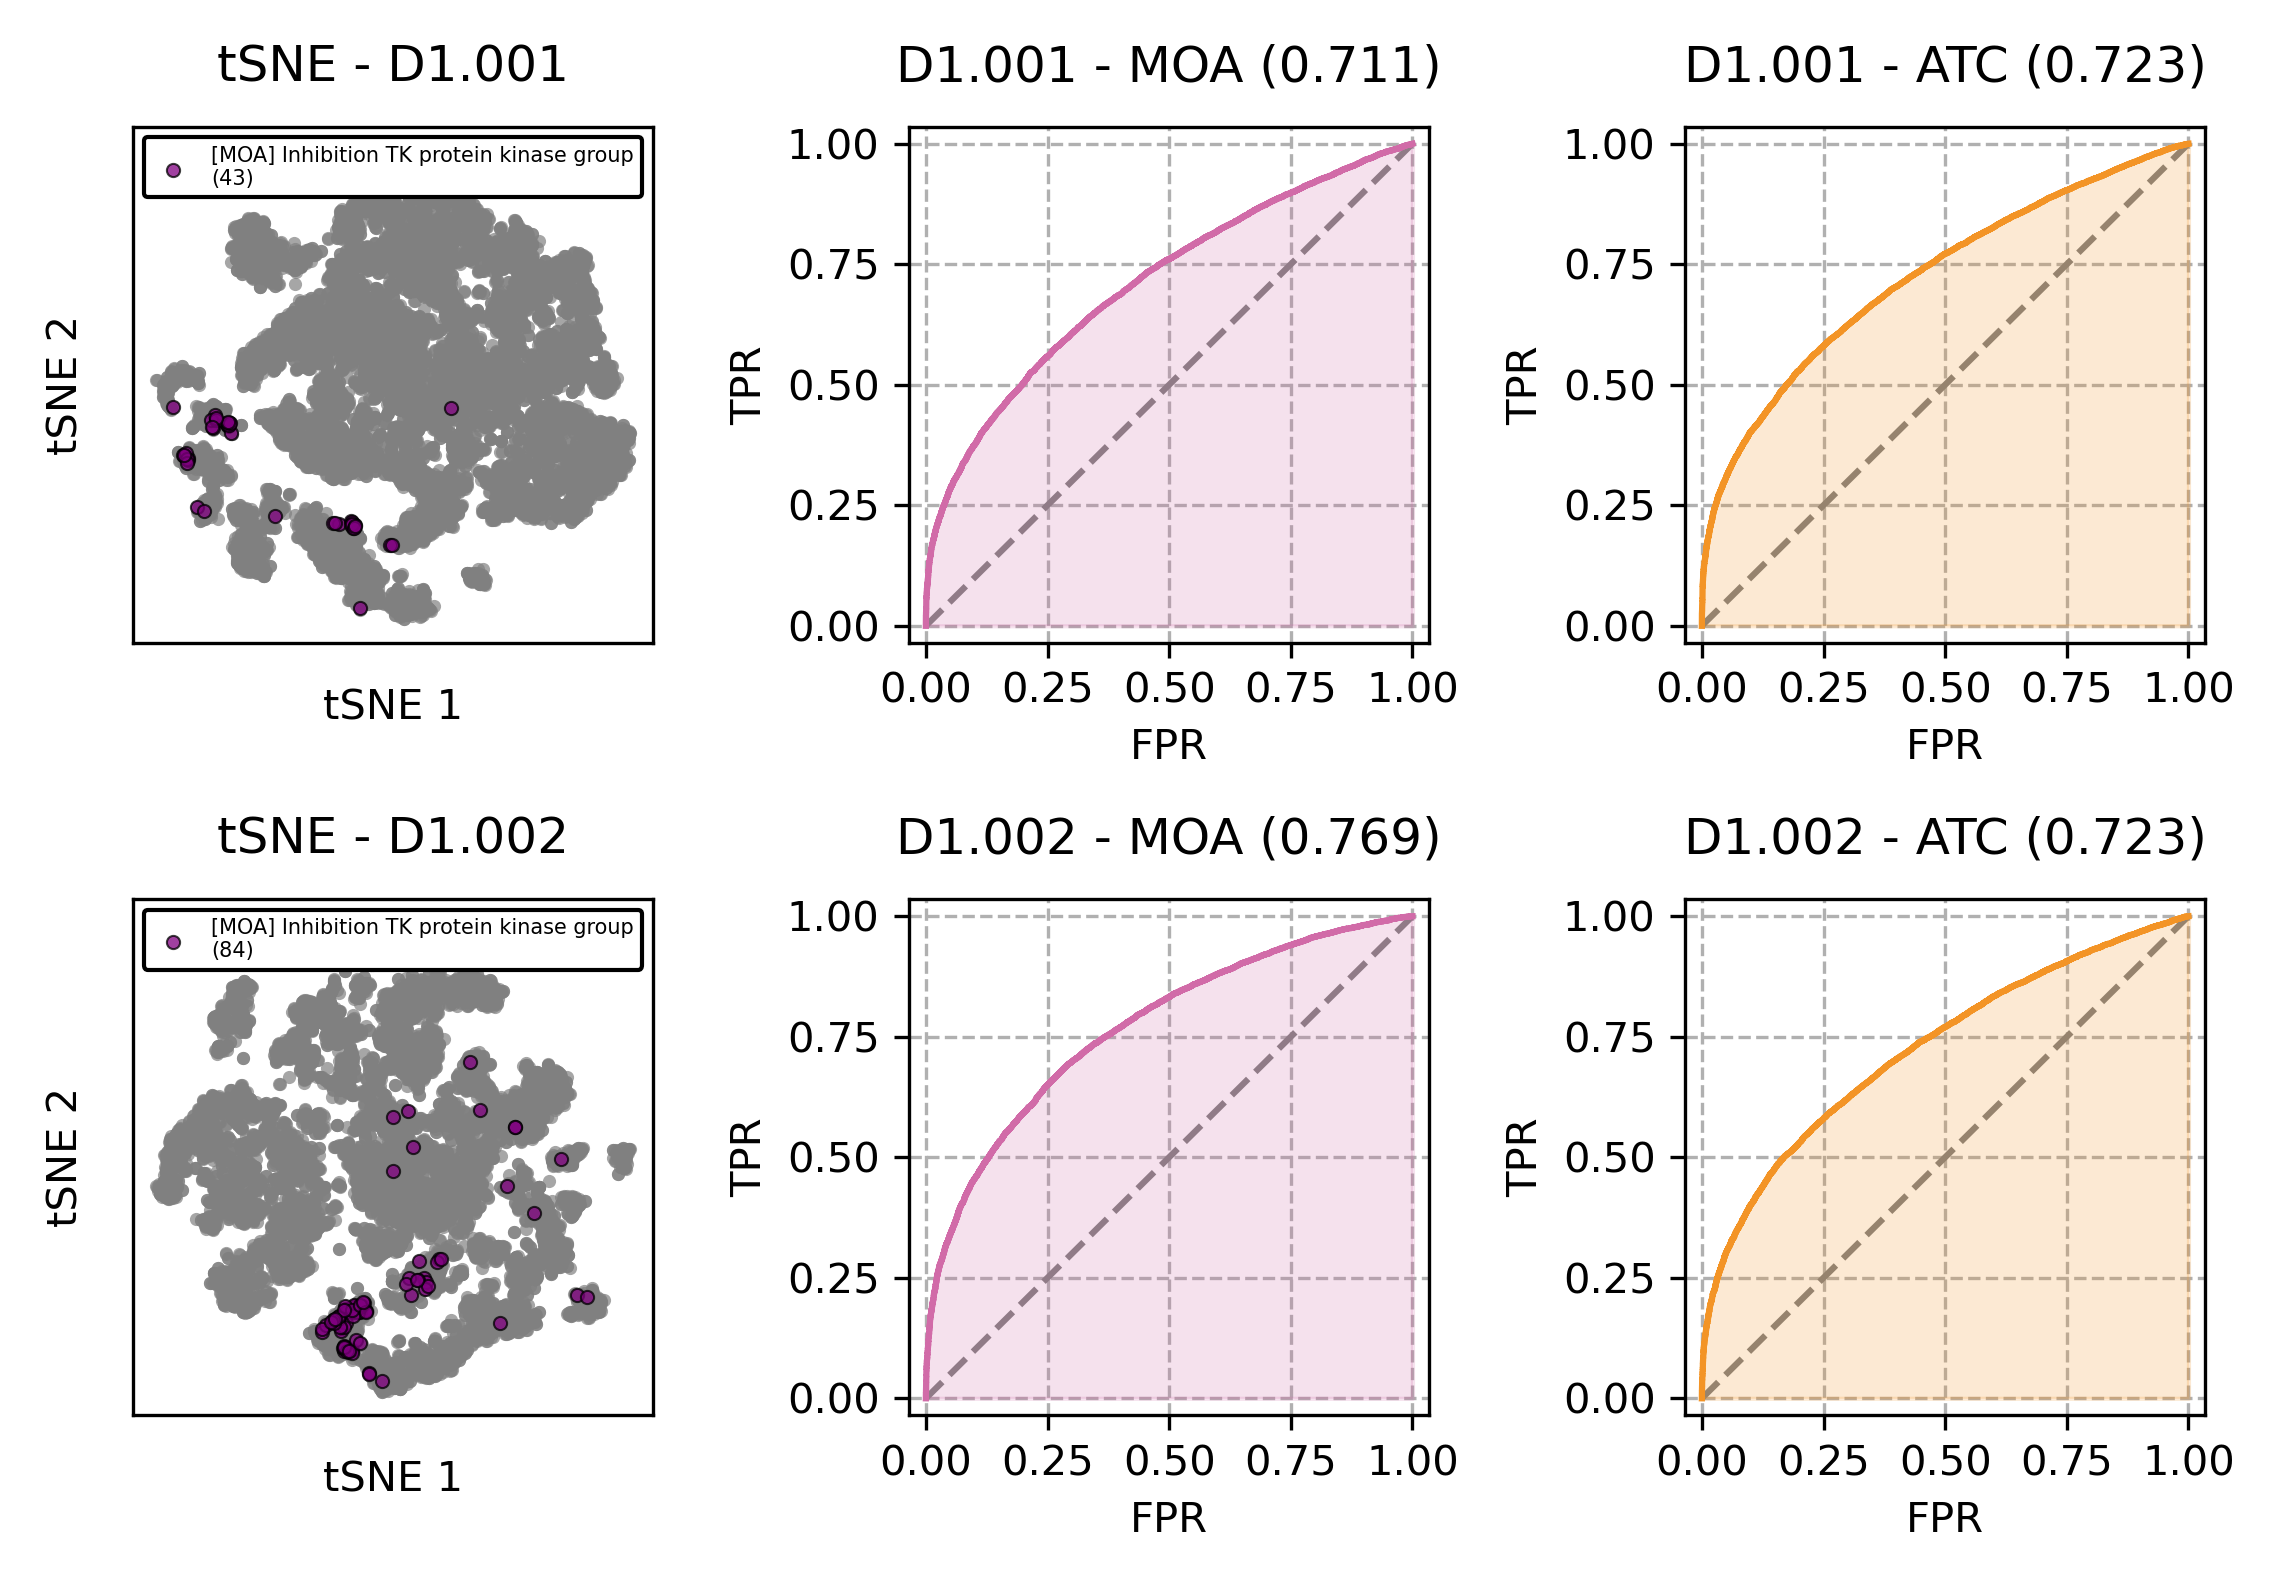
\includegraphics[width=1\linewidth]{figures/Protocols/Supplementary/FigS6.png}
  \caption{
    Comparison between D1.001 and D1.002. Left: 2D tSNE representation of D1.001 (top) and D1.002 (bottom) type III signatures having a corresponding type 0 signature in D1.001 and D1.002, respectively. Points highlighted in purple correspond to compounds related to the inhibition of the TK protein group.  Center and right: recapitulation of MOA (B1.001 type 0 signatures, purple) and ATC (E1.001 type 0 signatures, orange) using D1.001 (top) and D1.002 (bottom) type III signatures.  
  }
  \label{Protocols_FigS6}
\end{figure}


\begin{figure}[htbp]
  \centering
  \includegraphics[width=1\linewidth]{figures/Protocols/Supplementary/D6.001_v2.png}
  \caption{
    Diagnosis plots for the D6.001 space
    \textbf{a)} type 0 signatures,
    \textbf{b)} type I signatures,
    \textbf{c)} type II signatures. For further information about diagnosis plots, please see the \hyperref[Supplementary_Protocols_Diagnosis]{Supplementary Information}.
  }
  \label{Protocols_FigS7}
\end{figure}


\begin{figure}[htbp]
  \centering
  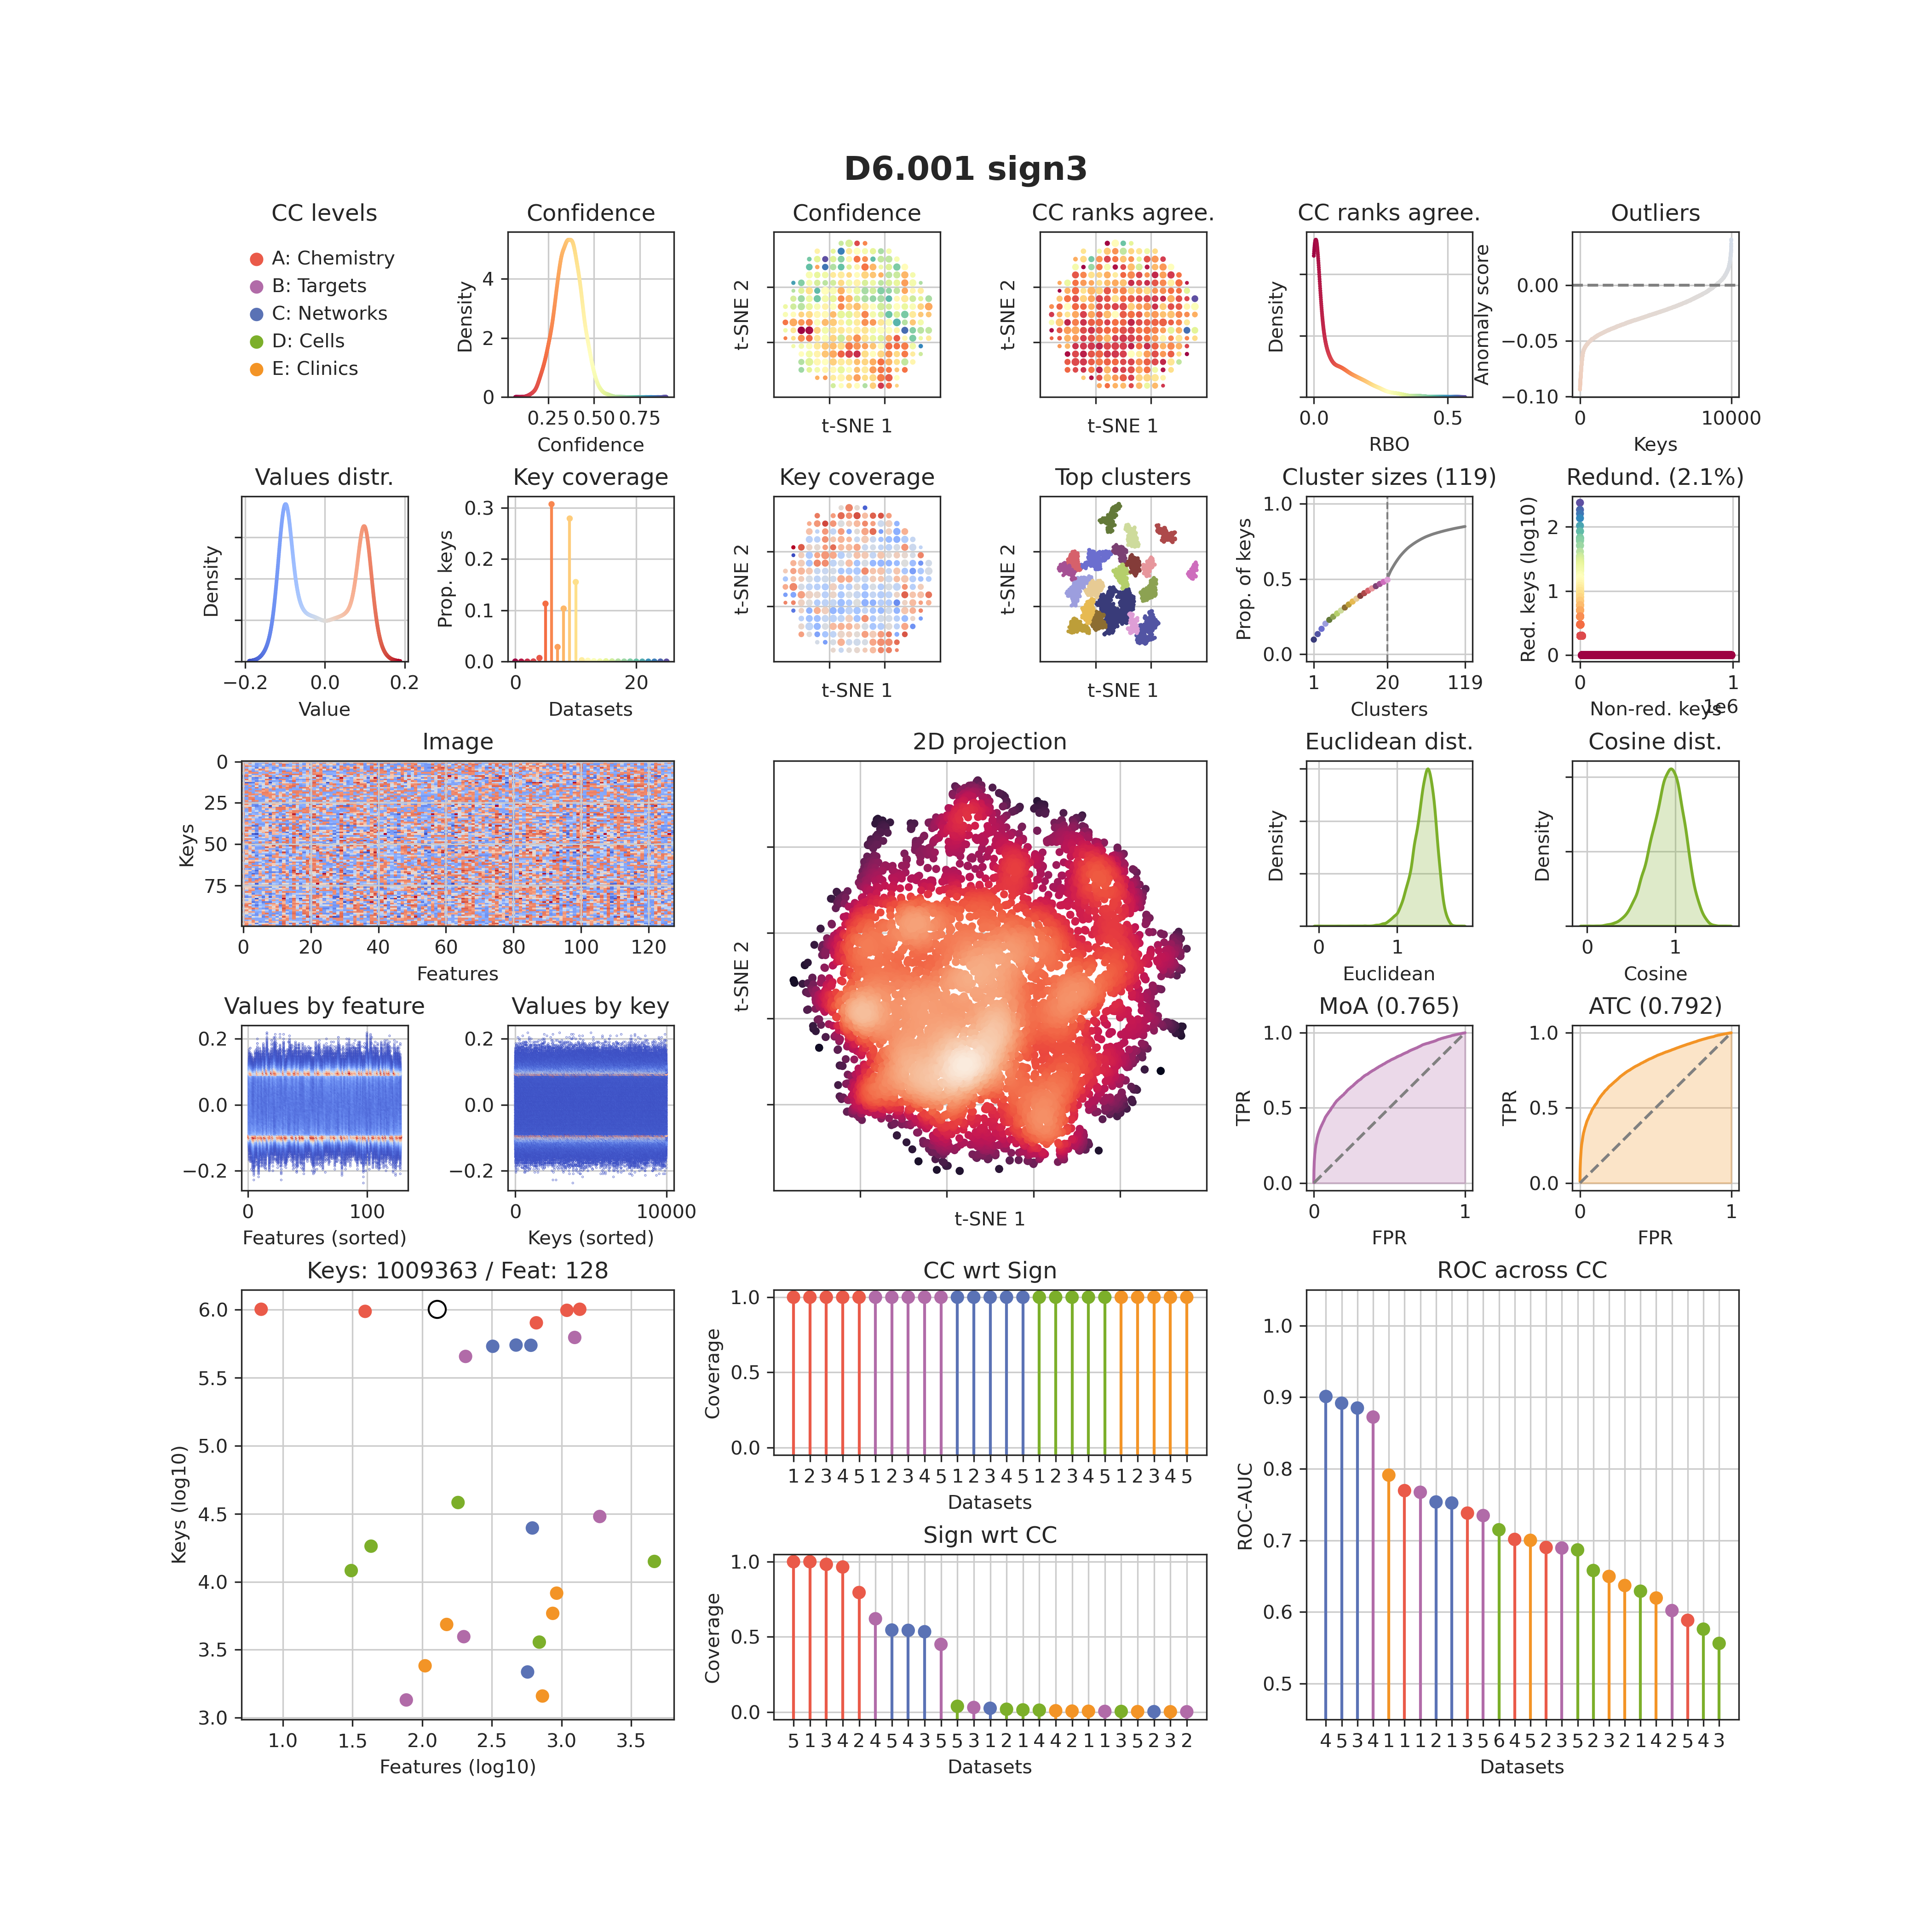
\includegraphics[width=1\linewidth]{figures/Protocols/Supplementary/D6.001_sign3_local_CC_D6_sign0_medium.png}
  \caption{
    Extended diagnosis plots for D6.001 type III signatures. For further information about diagnosis plots, please see the \hyperref[Supplementary_Protocols_Diagnosis]{Supplementary Information} and check our \href{https://gitlabsbnb.irbbarcelona.org/packages/protocols}{Gitlab repository}.
  }
  \label{Protocols_FigS8}
\end{figure}


\begin{figure}[htbp]
  \centering
  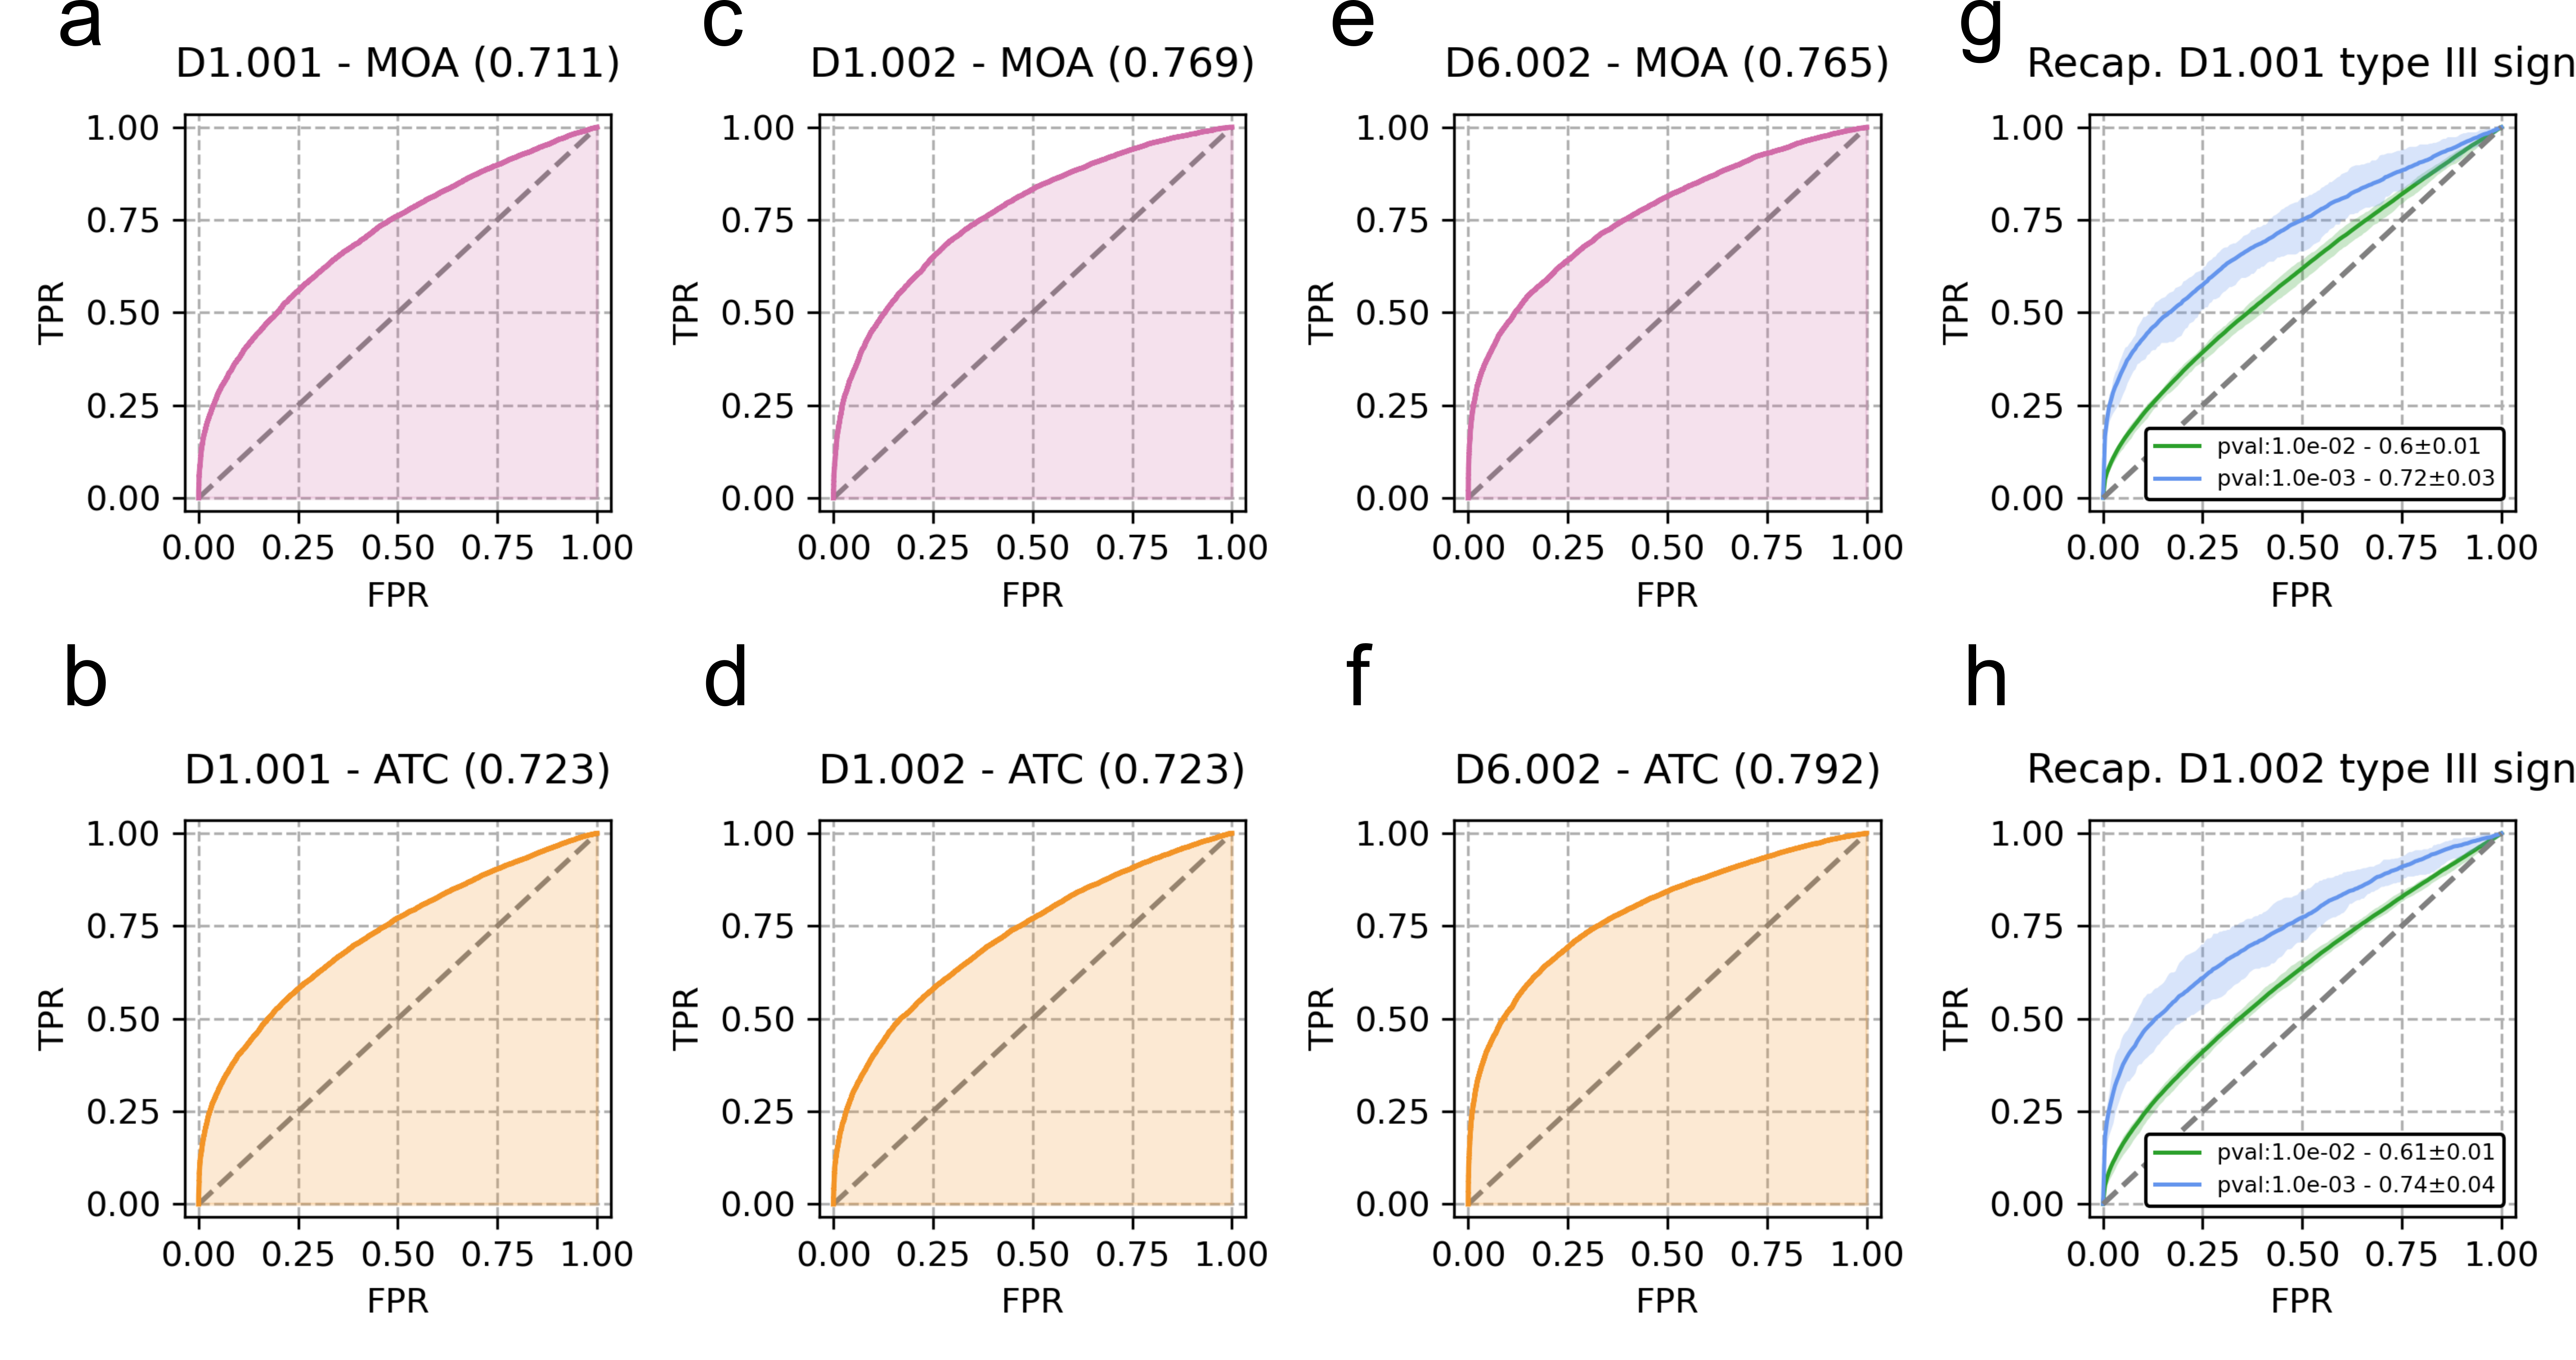
\includegraphics[width=1\linewidth]{figures/Protocols/Supplementary/FigS9_v2.png}
  \caption{
    Comparison between D1.001, D1.002 and D6.001.
    \textbf{a)} Recapitulation of MoA (B1.001 type 0 signatures, purple) using D1.001 type III signatures.
    \textbf{b)} Recapitulation of ATC (E1.001 type 0 signatures, orange) using D1.001 type III signatures.
    \textbf{c)} Recapitulation of MoA (B1.001 type 0 signatures, purple) using D1.002 type III signatures.
    \textbf{d)} Recapitulation of ATC (E1.001 type 0 signatures, orange) using D1.002 type III signatures. 
    \textbf{e)} Recapitulation of MoA (B1.001 type 0 signatures, purple) using D6.001 type III signatures.
    \textbf{f)} Recapitulation of ATC (E1.001 type 0 signatures, orange) using D6.001 type III signatures.
    \textbf{g)} Recapitulation of kNN at D1.001 type III signature level using D6.001 type III signatures at p-values 0.01 and 0.001.
    \textbf{h)} Recapitulation of NN at D1.002 type III signature level using D6.001 type III signatures at p-values 0.01 and 0.001.
  }
  \label{Protocols_FigS9}
\end{figure}


\begin{figure}[htbp]
  \centering
  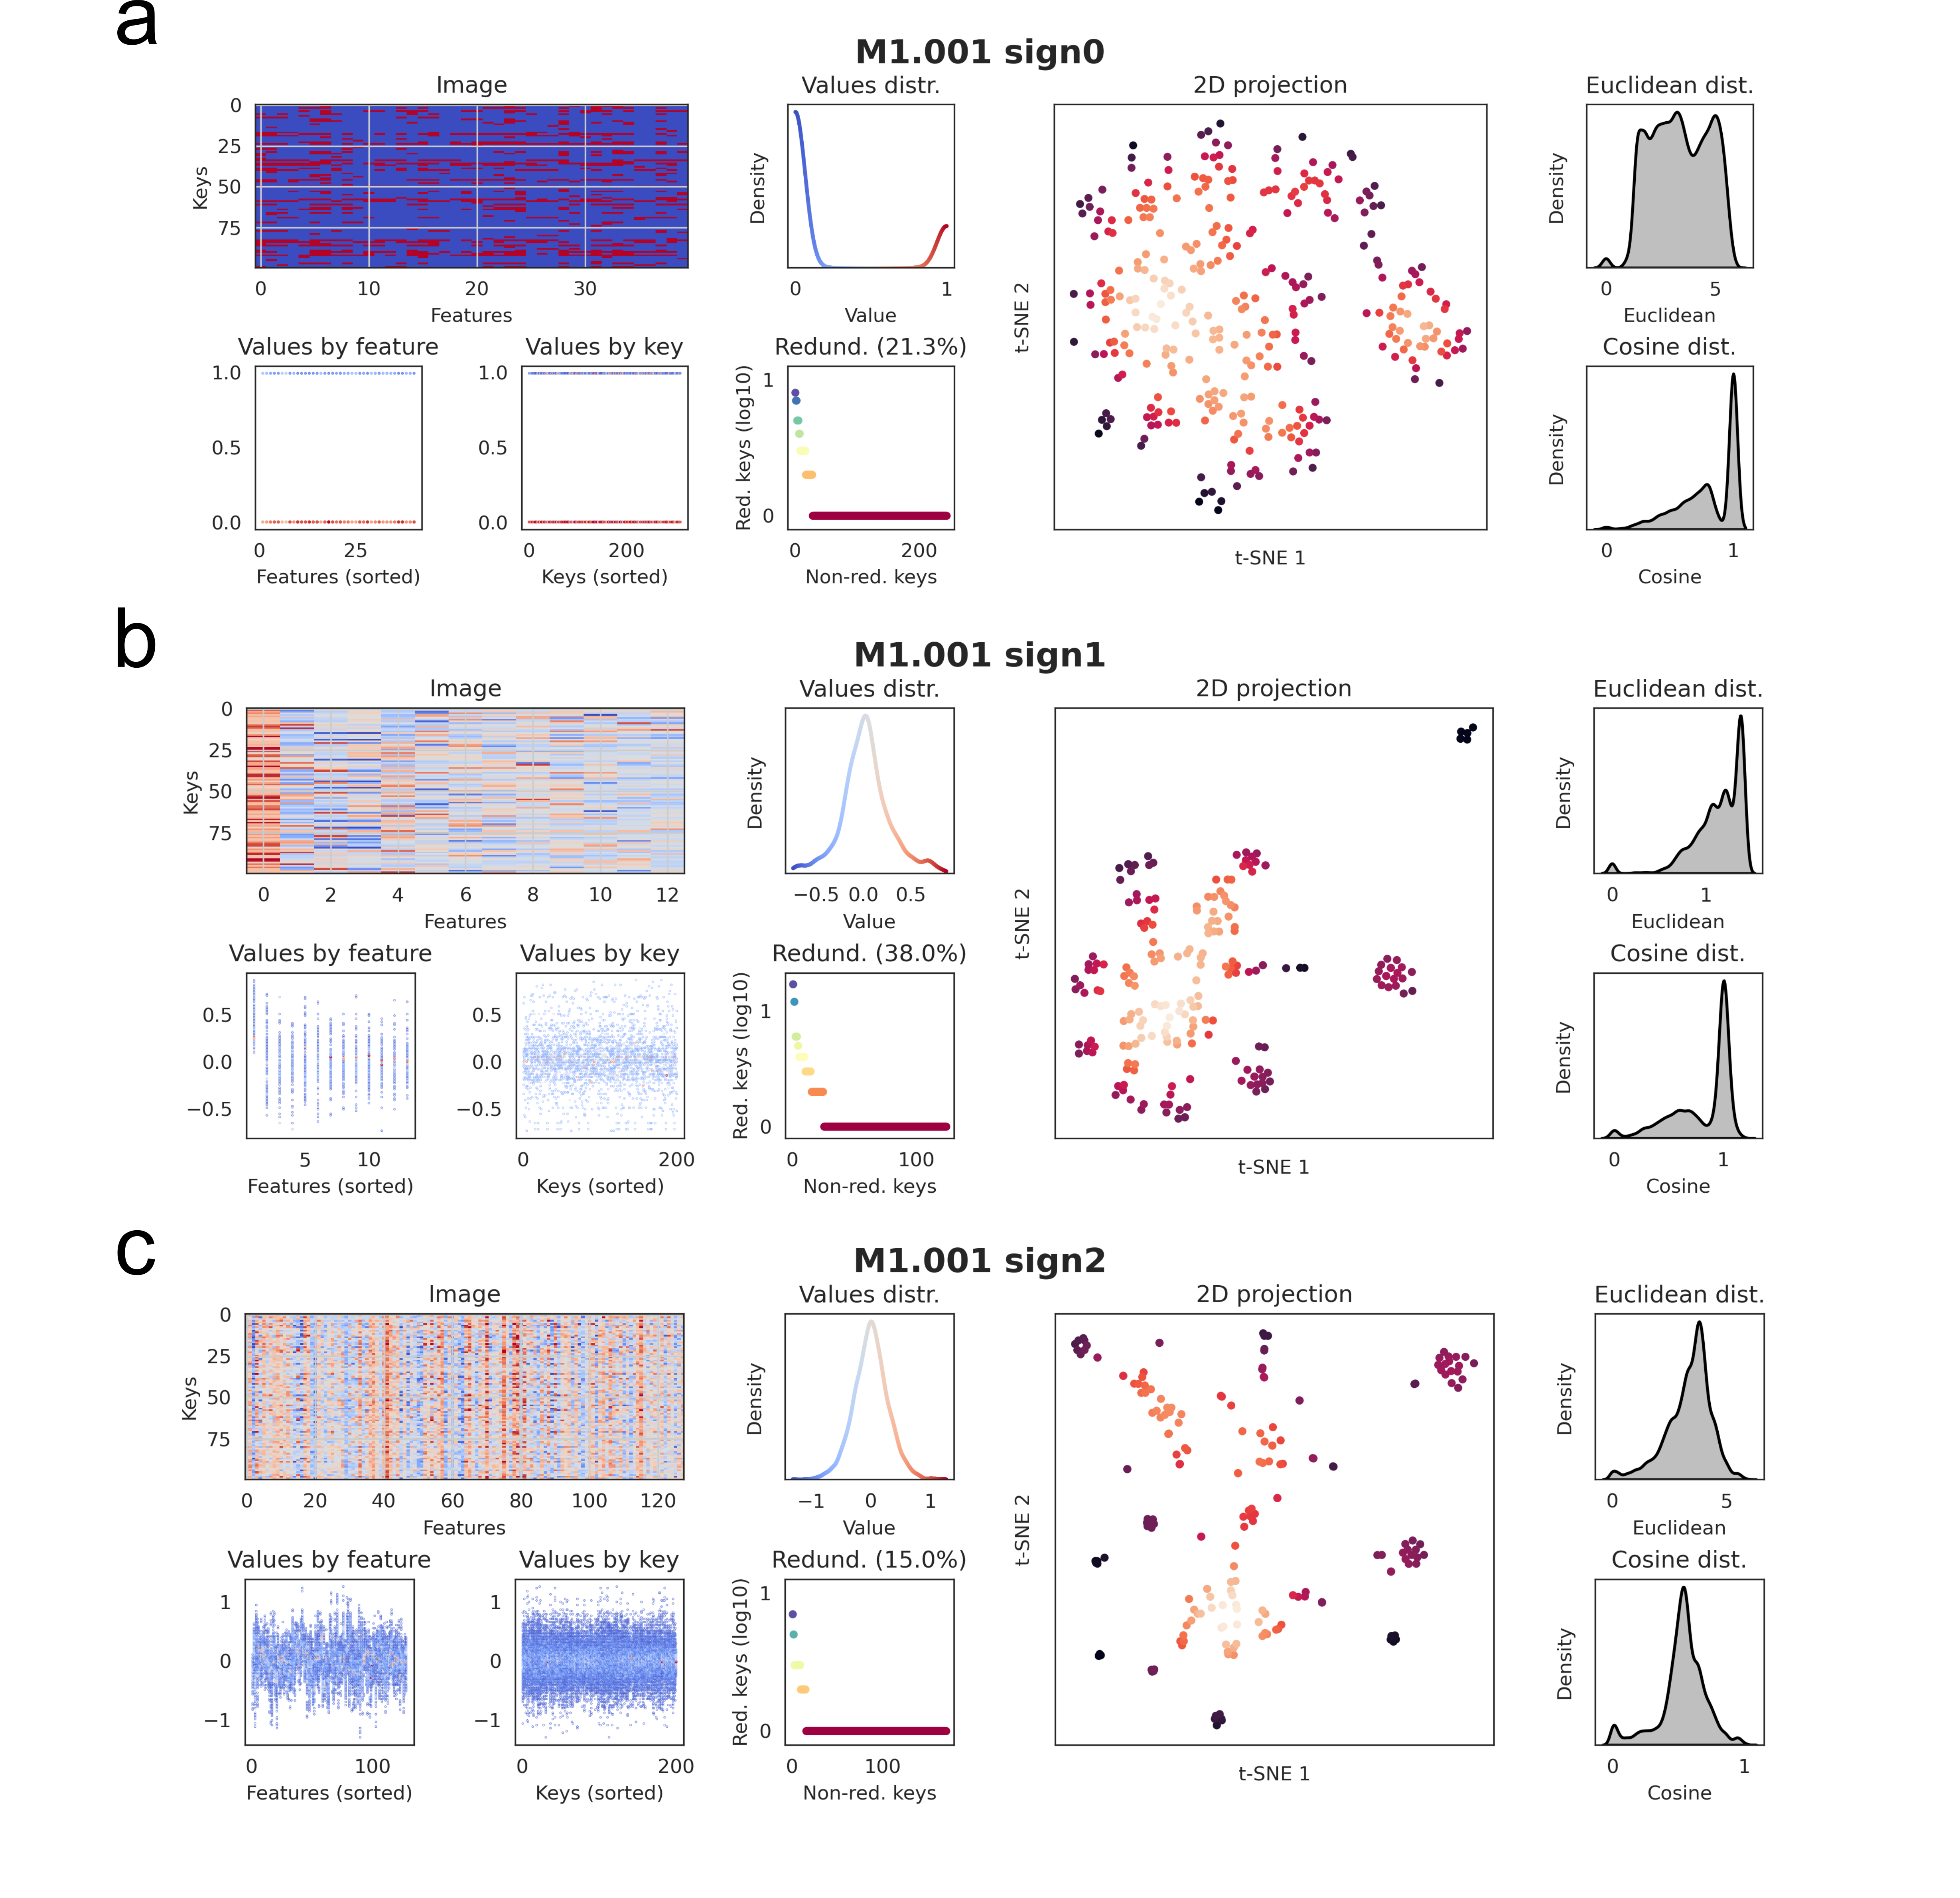
\includegraphics[width=1\linewidth]{figures/Protocols/Supplementary/M1.001_v2.png}
  \caption{
    Diagnosis plots for the M1.001 space
    \textbf{a)} type 0 signatures,
    \textbf{b)} type I signatures,
    \textbf{c)} type II signatures. For further information about diagnosis plots, please see the \hyperref[Supplementary_Protocols_Diagnosis]{Supplementary Information}.
  }
  \label{Protocols_FigS10}
\end{figure}

\begin{figure}[htbp]
  \centering
  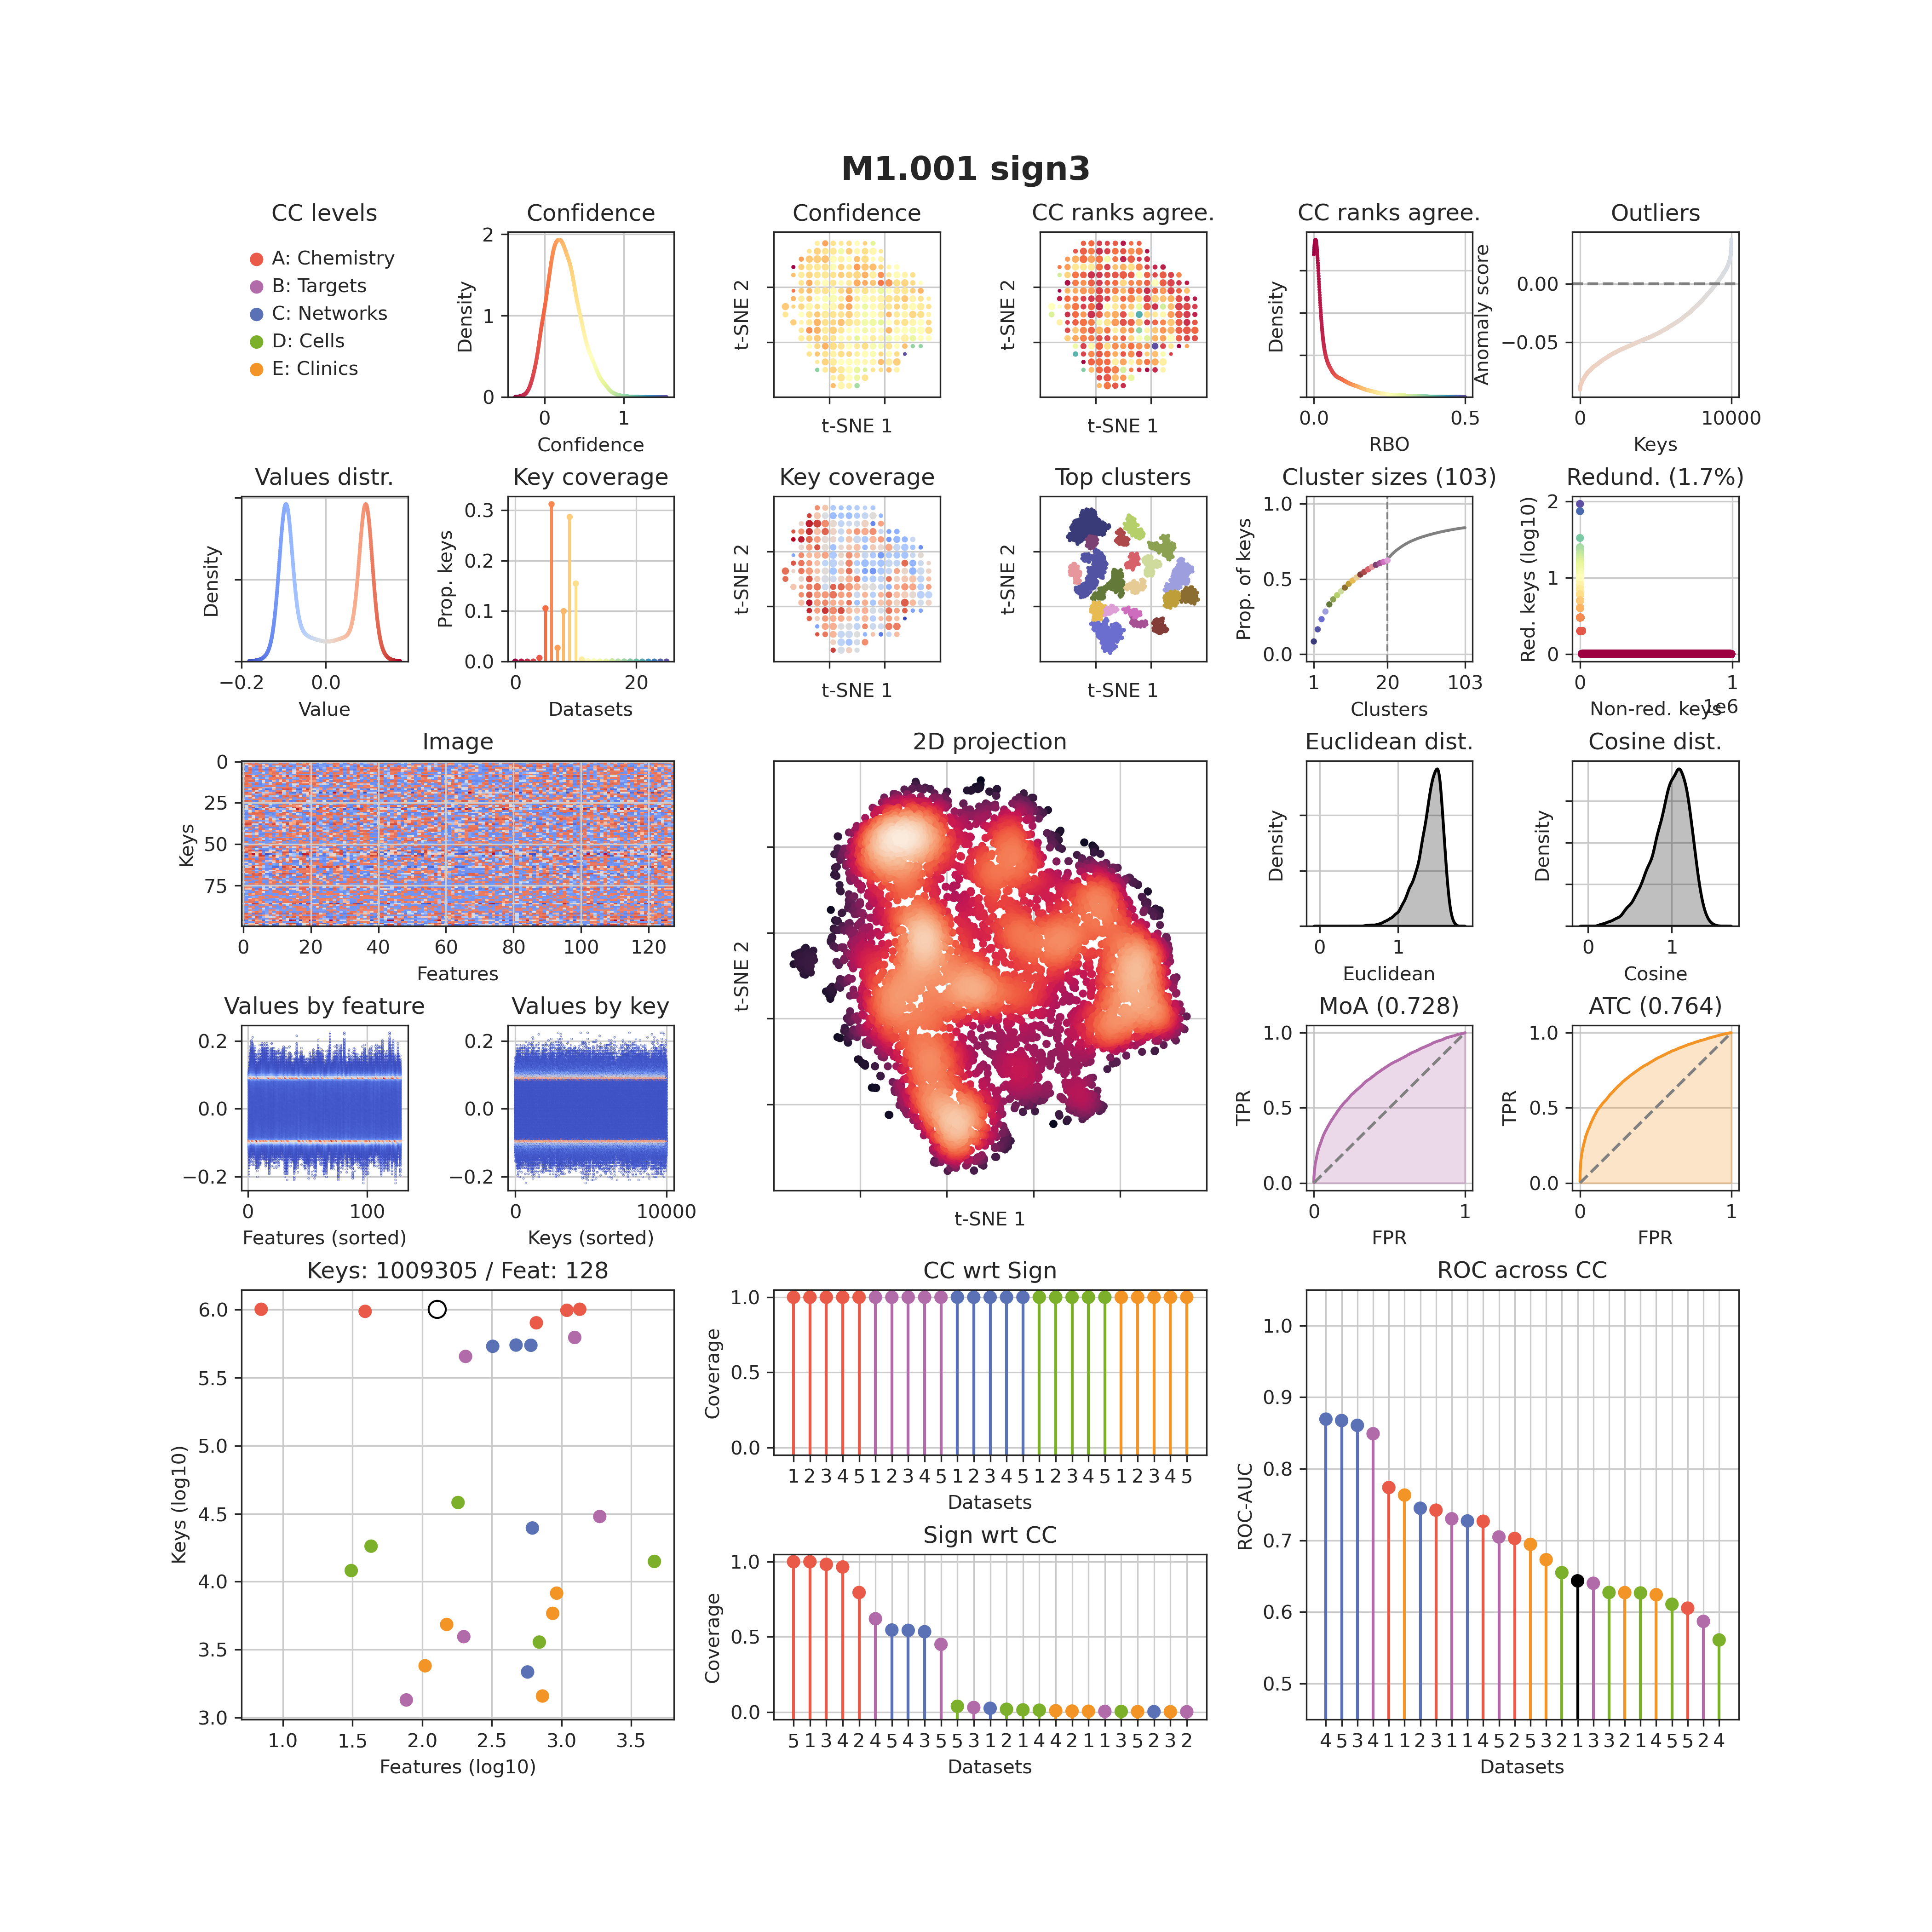
\includegraphics[width=1\linewidth]{figures/Protocols/Supplementary/M1.001_sign3_local_CC_M1_sign0_medium.png}
  \caption{
    Extended diagnosis plots for M1.001 type III signatures. For further information about diagnosis plots, please see the \hyperref[Supplementary_Protocols_Diagnosis]{Supplementary Information} and check our \href{https://gitlabsbnb.irbbarcelona.org/packages/protocols}{Gitlab repository}.
  }
  \label{Protocols_FigS11}
\end{figure}



\phantomsection
\subsection{Interpreting the results: diagnosis plots}
\label{Supplementary_Protocols_Diagnosis}







\phantomsection
\subsection{Supplementary Code}

\phantomsection
\subsubsection{Main Protocol}

\begin{lstlisting}
# This is a sample Python code
def hello_world():
    print("Hello, World!")

hello_world()
\end{lstlisting}